% \documentclass{article}

%%v helpful MIT exam schema, see http://www-math.mit.edu/~psh/exam/examdoc.pdf
 \documentclass[8pt]{exam} 
% \qformat{\textbf{Question \thequestion}\quad \thepoints\hfill } % Large depth to make space}
 \renewcommand{\thesubpart}{(\roman{subpart})}
 \renewcommand{\subpartlabel}{\thesubpart}
 \footer{}{}{Page \thepage\ de \numpages}
\addpoints
% \pointsinmargin
% \boxedpoints
\renewcommand{\questionshook}{\setlength{\itemsep}{1mm}}
\renewcommand{\partshook}{
	\setlength{\itemsep}{0.1cm}
}

\usepackage{cmbright}

\pagestyle{empty} %for handouts
\addtolength{\jot}{2em} % this makes all formulae a bit more spaced vertically for handouts
\setlength{\parindent}{0pt} %we're not writing a novel
%\renewcommand{\arraystretch}{2} %makes tables taller, so easier to write in

\usepackage{amsmath, amssymb} %standard classy maths symbols
\usepackage[a4paper, margin=1in]{geometry} %makes it easy to specify where to put stuff on the page

\usepackage{siunitx} %v handy way of getting SI units to typeset correctly...
\sisetup{locale = FR} %... and now it will use a comma for decimals
\usepackage{icomma}

\usepackage[utf8]{inputenc}

%\usepackage[french]{babel} % frenchify everything (e.g. a Table becomes a Tableau)
%\usepackage{lmodern} % font with nicer French characters than standard
%\usepackage{textcomp} % and more help for special characters

\usepackage{tcolorbox} % basic but good package for boxes around text
\tcbset{colback=black!2!white}
\usepackage{color} % colours
%\newcommand{\fillin}{\color{black!1!white}} %makes the text disappear
%\definecolor{fillin}{rgb} {1.00,1.00,1.00}
%\renewcommand{\fillin}{\color{blue}} \definecolor{fillin}{rgb} {0.00,0.00,1.00} %makes the filling in text appear (in blue)

\usepackage{enumitem} % can change the labels on lists, items, enumerates

\usepackage{tikz, pgfplots} % interval diagrams, sets, etc.
\usetikzlibrary{calc,trees,positioning,arrows,fit,shapes,calc,angles,quotes}

\pgfplotsset{every axis/.append style={
axis x line=middle,    % put the x axis in the middle
axis y line=middle,    % put the y axis in the middle
axis line style={->}, % arrows on the axis
title={},
xlabel={$x$},          % default put x on x-axis
ylabel={$y$},          % default put y on y-axis
ticks=none
}}

\begin{document}

\textbf{Name:} \dotfill

\

$\triangle ABC$ is placed against a right-angled corner $O$ such that $AB$ bisects $\widehat{CAM}$ and $BC$ bisects $\widehat{NCA}$. \\
Let $x = B\hat{A}C$ and $y= B\hat{C}A$.

\begin{center}
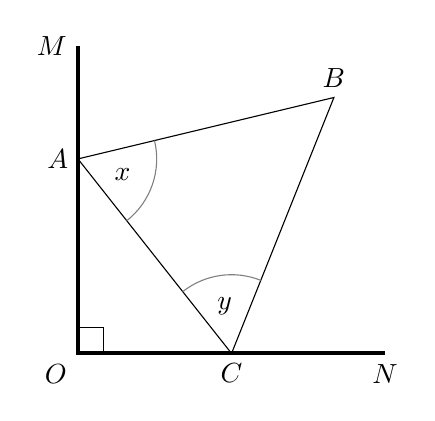
\begin{tikzpicture}[scale=1.3]
  \coordinate (A) at (0,1.9);
  \coordinate (B) at (2.5,2.5);
  \coordinate (C) at (1.5,0);
  \draw[line width=0.5mm] (3,0) node[below] {$N$} --  (0,0) node[below left] {$O$} --  (0,3) node[left] {$M$};
  \draw (0,0) +(.25,0) |- +(0,.25);
%  \draw (10,0) --  (0,0) -- node[right] {15 cm} (0,10);
  \draw (C) node[below] {$C$} --  (B) node[above] {$B$} -- (A) node[left] {$A$}  -- cycle;
\pic [angle radius=1cm, draw=gray,"$y$"] {angle=B--C--A};
\pic [angle radius=1cm, draw=gray, "$x$" ] {angle=C--A--B};
\end{tikzpicture}
\end{center}

\begin{questions}


\question[1] Explain why $B\hat{A}M = x $.
\fillwithdottedlines{7mm}

\question[2] Calculate $O\hat{A}C$ in terms of $x$.
\fillwithdottedlines{7mm}

\question[3] By considering the angles of $\triangle OAC$ find an equation relating $x$ and $y$.
\fillwithdottedlines{28mm}

\question[2] Explaining your reasoning, find $A\hat{B}C$.
\fillwithdottedlines{63mm}


\end{questions}

\textbf{Bonus:} Overleaf, prove that the angle bisectors of any given triangle intersect!

\vfill 

\begin{tcolorbox}

\textbf{Name of corrector:}

\begin{center}
\gradetable[h][questions]
\end{center}

\end{tcolorbox}

\end{document}